
Our empirical evaluation of Standard Conformal Prediction (SCP), Time-Weighted Conformal Prediction (TWCP), and QUPEC across four datasets is summarized in Table \ref{tab:results_comparison}. Performance is assessed on the Expected Daily Coverage Gap (a proxy for reliability) and Average Interval Width (efficiency), with lower values being better for both.

\textbf{The results highlight QUPEC's consistent ability to minimize the coverage gap.} This improvement in reliability generally comes at the cost of wider prediction intervals. For instance, QUPEC nearly eliminates the coverage gap for the Online Retail dataset, but at the cost of a 32\% increase in interval width compared to SCP.

Strikingly, for the Elo dataset, QUPEC improves both reliability and efficiency, reducing the coverage gap by over 64\% while also narrowing the prediction intervals. This demonstrates QUPEC's adaptability to varied data structures.

In contrast, TWCP's performance is limited, offering an improvement over SCP only on the Amazon dataset. Notably, for the Online Retail, The Complete Journey, and Elo datasets, TWCP provided no advantage, underscoring that temporal weighting alone is often insufficient for panel data. This highlights the critical need to account for panel heterogeneity, a key feature of QUPEC. The dataset-dependent nature of the results, reflected in the optimal hyperparameters, confirms that the balance between temporal and cross-sectional factors varies significantly across different contexts.

\begin{table*}[t]
\centering
\caption{Expected Daily Coverage Gap and Average Interval Width. For TWCP and QUPEC, results correspond to the hyperparameters $(\beta_{time}, \beta_{entity})$ that minimized the coverage gap. Lower values are better for both metrics.}
\label{tab:results_comparison}
\begin{tabular}{|l|cc|cc|cc|}
\hline
\multirow{2}{*}{\textbf{Dataset}} & \multicolumn{2}{c|}{\textbf{Standard Conformal}} & \multicolumn{2}{c|}{\textbf{Time-Weighted Conformal}} & \multicolumn{2}{c|}{\textbf{QUPEC}} \\
\cline{2-7}
& \textbf{Gap} & \textbf{Width} & \textbf{Gap} & \textbf{Width} & \textbf{Gap} & \textbf{Width} \\
\hline
Amazon & 0.0197 & \textbf{0.1826} & 0.0160 & 0.1898 & \textbf{0.0137} & 0.2022 \\
Online Retail & 0.0035 & \textbf{0.1043} & 0.0035 & 0.1043 & \textbf{0.0000} & 0.1378 \\
The Complete Journey & 0.0141 & \textbf{0.2505} & 0.0141 & 0.2505 & \textbf{0.0131} & 0.2566 \\
Elo & 0.0028 & 0.2072 & 0.0028 & 0.2072 & \textbf{0.0010} & \textbf{0.2042} \\
\hline
\end{tabular}
\end{table*}

\begin{figure*}[t]
    \centering
    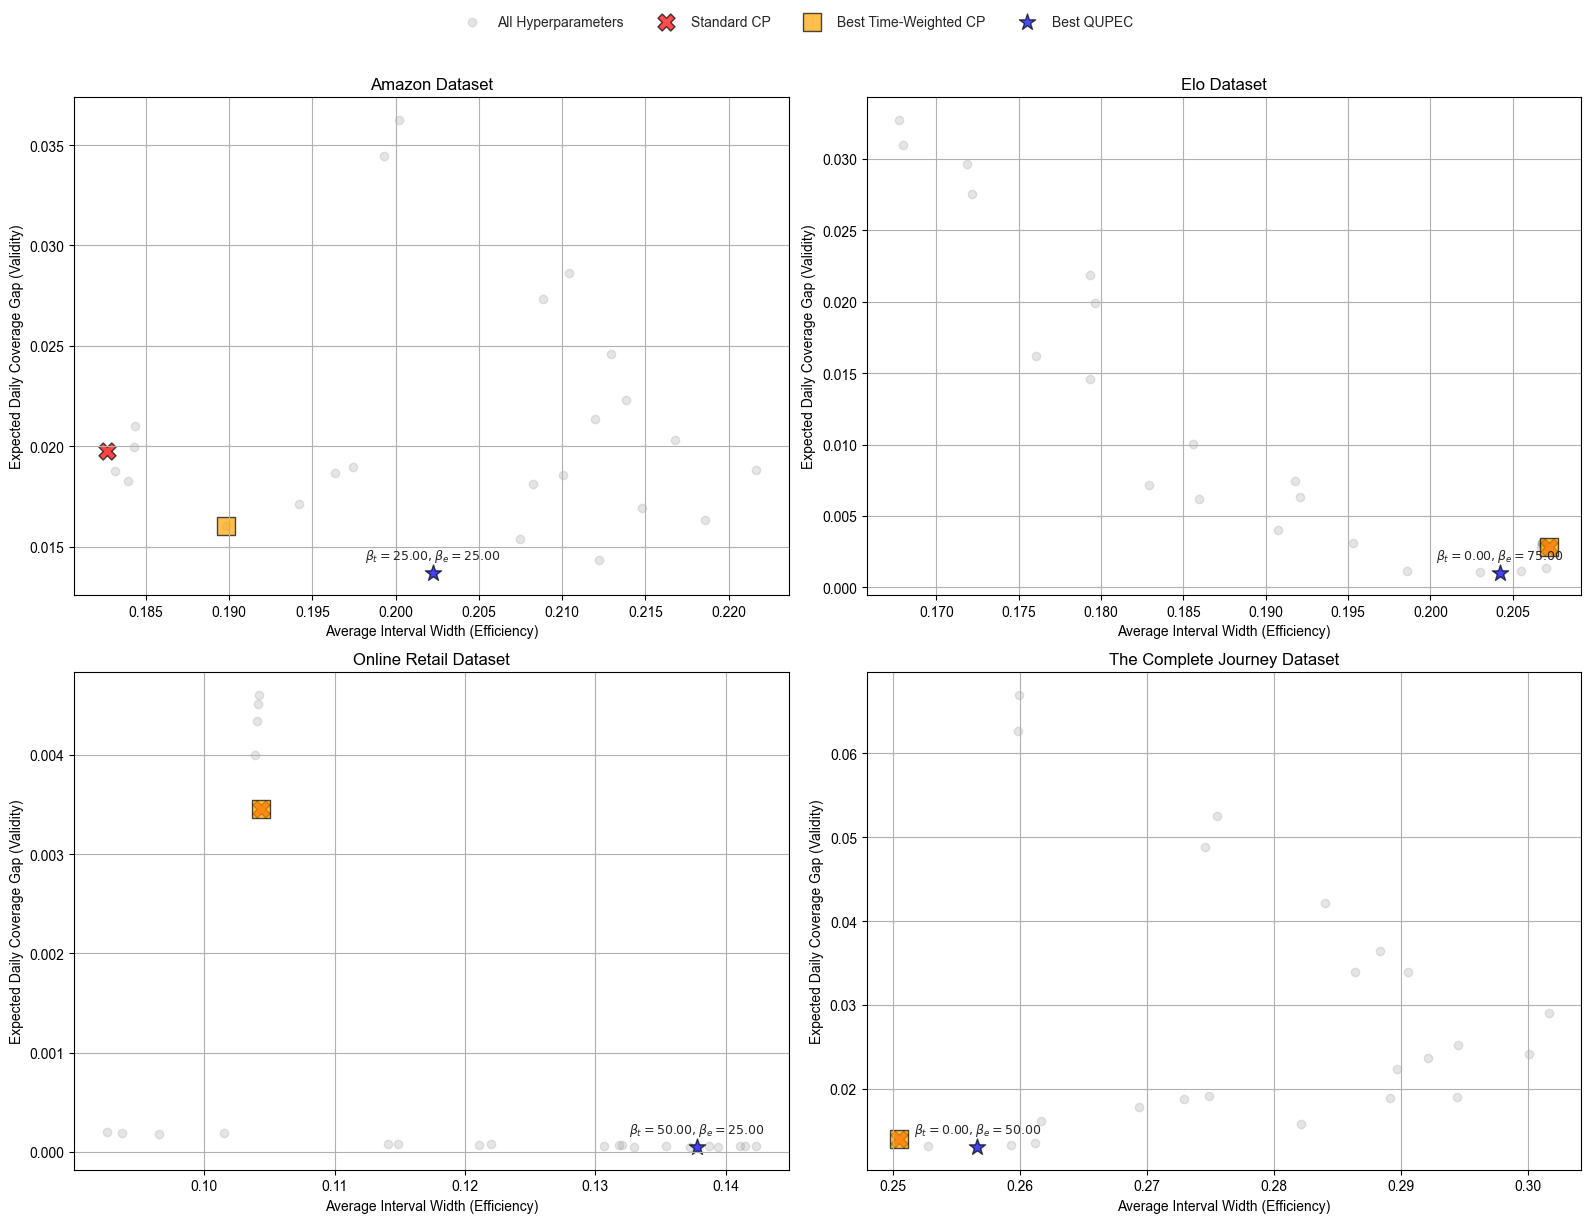
\includegraphics[width=\linewidth]{images/tradeoff_plots_combined.png}
    \caption{Comparison of Validity-Efficiency Trade-off for All Datasets.}
    \label{fig:tradeoff_plots_combined}
\end{figure*}
